
\documentclass[landscape,a0paper,fontscale=.235]{xebaposter} % Adjust the font scale/size here

\usepackage{relsize}	% Control relative text size 
\usepackage{wrapfig}  % Wrap text around figure
\usepackage{graphicx} % Required for including images

\usepackage{amsmath} % For typesetting math
\usepackage{amssymb} % Adds new symbols to be used in math mode

\usepackage{booktabs} % Top and bottom rules for tables
\usepackage{enumitem} % Used to reduce itemize/enumerate spacing
\newlist{todolist}{itemize}{1}
\setlist[todolist]{label=$\square$}

\usepackage{palatino} % Use the Palatino font
\usepackage[font=small,labelfont=bf]{caption} % Required for specifying captions to tables and figures

\usepackage{multicol} % Required for multiple columns
\setlength{\columnsep}{1.5em} % Slightly increase the space between columns
\setlength{\columnseprule}{0mm} % No horizontal rule between columns

\definecolor{lightblue}{rgb}{0.145,0.6666,1} % Defines the color used for content box headers

\begin{document}

\begin{poster}
{
columns=4, % number of columns
headerborder=closed, % Adds a border around the header of content boxes
colspacing=1em, % Column spacing
%bgColorOne=white, % Background color for the gradient on the left side of the poster
%bgColorTwo=white, % Background color for the gradient on the right side of the poster
background=none, % no background colour
borderColor=lightblue, % Border color
headerColorOne=black, % Background color for the header in the content boxes (left side)
headerColorTwo=lightblue, % Background color for the header in the content boxes (right side)
headerFontColor=white, % Text color for the header text in the content boxes
boxColorOne=white, % Background color of the content boxes
textborder=roundedleft, % Format of the border around content boxes, can be: none, bars, coils, triangles, rectangle, rounded, roundedsmall, roundedright or faded
eyecatcher=true, % Set to false for ignoring the left logo in the title and move the title left
headerheight=0.14\textheight, % Height of the header
headershape=roundedright, % Specify the rounded corner in the content box headers, can be: rectangle, small-rounded, roundedright, roundedleft or rounded
headerfont=\Large\bf\textsc, % Large, bold and sans serif font in the headers of content boxes
%textfont={\setlength{\parindent}{1.5em}}, % Uncomment for paragraph indentation
linewidth=.75pt % Width of the border lines around content boxes
}
%----------------------------------------------------------------------------------------
%	TITLE SECTION 
%----------------------------------------------------------------------------------------
% LEFT LOGOS
{
\setlength\fboxsep{0pt}
\setlength\fboxrule{0pt}
	\fbox{
		\begin{minipage}{8em}
			\includegraphics[width=4.5em,height=4.5em]{cpl_logo.png}
			\includegraphics[width=5em,height=4em]{mps_logo.png}
		\end{minipage}
	}
}
% TITLE & AUTHORS
{\bf\textsc{\emph{restingIAF}: a reliable, automated method for quantifying Individual Alpha Frequency}\vspace{.2em}} % Poster title
{\smaller Andrew W. Corcoran\textsuperscript{a,b} Phillip M. Alday\textsuperscript{c,b} Matthias Schlesewsky\textsuperscript{b} Ina Bornkessel-Schlesewsky\textsuperscript{b}} % Author names
% RIGHT LOGOS
{
\setlength\fboxsep{0pt}
\setlength\fboxrule{0pt}
	\fbox{
		\begin{minipage}{8em}
			\includegraphics[width=4em,height=5em]{cnl_logo.png}
			\includegraphics[width=4em,height=5em]{unisa_logo.png}
		\end{minipage}
	}
}


%----------------------------------------------------------------------------------------
%	MAIN BODY - LEFT COLUMN
%----------------------------------------------------------------------------------------

\headerbox{Introduction}{name=intro,column=0,row=0}{
\textbf{IAF} is a fundamental property of brain processing relating to individual differences across various domains:
\begin{itemize}[noitemsep]
\item perception\textsuperscript{[1,2]}
\item memory\textsuperscript{[3]} \& attention\textsuperscript{[4]}
\item language\textsuperscript{[5]}
\item general intelligence\textsuperscript{[6]}
\end{itemize}
IAF might also help improve the precision of frequency band analysis.\textsuperscript{[7]}

\vspace{0.3em} % When there are two boxes, some whitespace may need to be added if the one on the right has more content
}

\headerbox{The Problem}{name=problem,column=1}{
IAF is typically indexed by a dominant spectral peak elicited during eyes-closed resting-state M/EEG. However, a subset of individuals do not demonstrate any clear alpha peak.
\\-- \textbf{Visual identification} of spectral peaks in such cases is inefficient, prone to bias, and difficult to replicate.
\\-- \textbf{Automated strategies} may solve these problems, but are themselves subject to various limitations.
}

\headerbox{The Idea}{name=idea,span=2,below=intro}{
We devised an automated routine that estimates \textbf{peak alpha frequency (PAF)} from the 1\textsuperscript{st} and 2\textsuperscript{nd} derivatives of \textbf{Savitzky-Golay (S-G) filtered} power spectra. 
\\S-G filtering smoothes noisy fluctuations while preserving peak characteristics.\textsuperscript{[8]}
\\We also extended this approach to derive \textbf{centre of gravity (CoG)} estimates of IAF.
}

\headerbox{Method \& Analysis}{name=method,span=2,below=idea}{
\begin{wrapfigure}{r}{.26\textwidth}
  \vspace*{-1cm}\includegraphics[height=7.4cm]{short_flow.pdf}
  %\caption{\smaller{Flow diagram summarising algorithm}}
\end{wrapfigure}

\textbf{\textsc{Algorithm}}
\\The routine is summarised in the flow diagram opposite.
\\To register as a PAF, peaks must exceed a background spectral noise threshold and a secondary peak threshold. Number of estimates for averaging can also be thresholded.
\\ \emph{restingIAF} has MATLAB and Python implementations.
\\[.25cm]
\textbf{\textsc{Empirical Data}}
\\63 healthy adults (42 females; age range: 18--74 yrs).
\\2 min eyes-closed EEG recorded pre/post experiment.
\\PAF/CoG distributions and correlations analysed.
\\[.25cm]
\textbf{\textsc{Simulation Data}}
\\Gaussian-distributed alpha components synthesised and embedded within a pink noise signal. Component dispersal (\textbf{$\alpha$}) and signal-to-noise ratio (\textbf{SNR}) parametrically varied. PAF/CoG compared to \textbf{local maximum (LM)} detection.

}

%----------------------------------------------------------------------------------------
%	MAIN BODY - RIGHT COLUMN
%----------------------------------------------------------------------------------------

\headerbox{Key Findings}{name=results,span=2,column=2}{

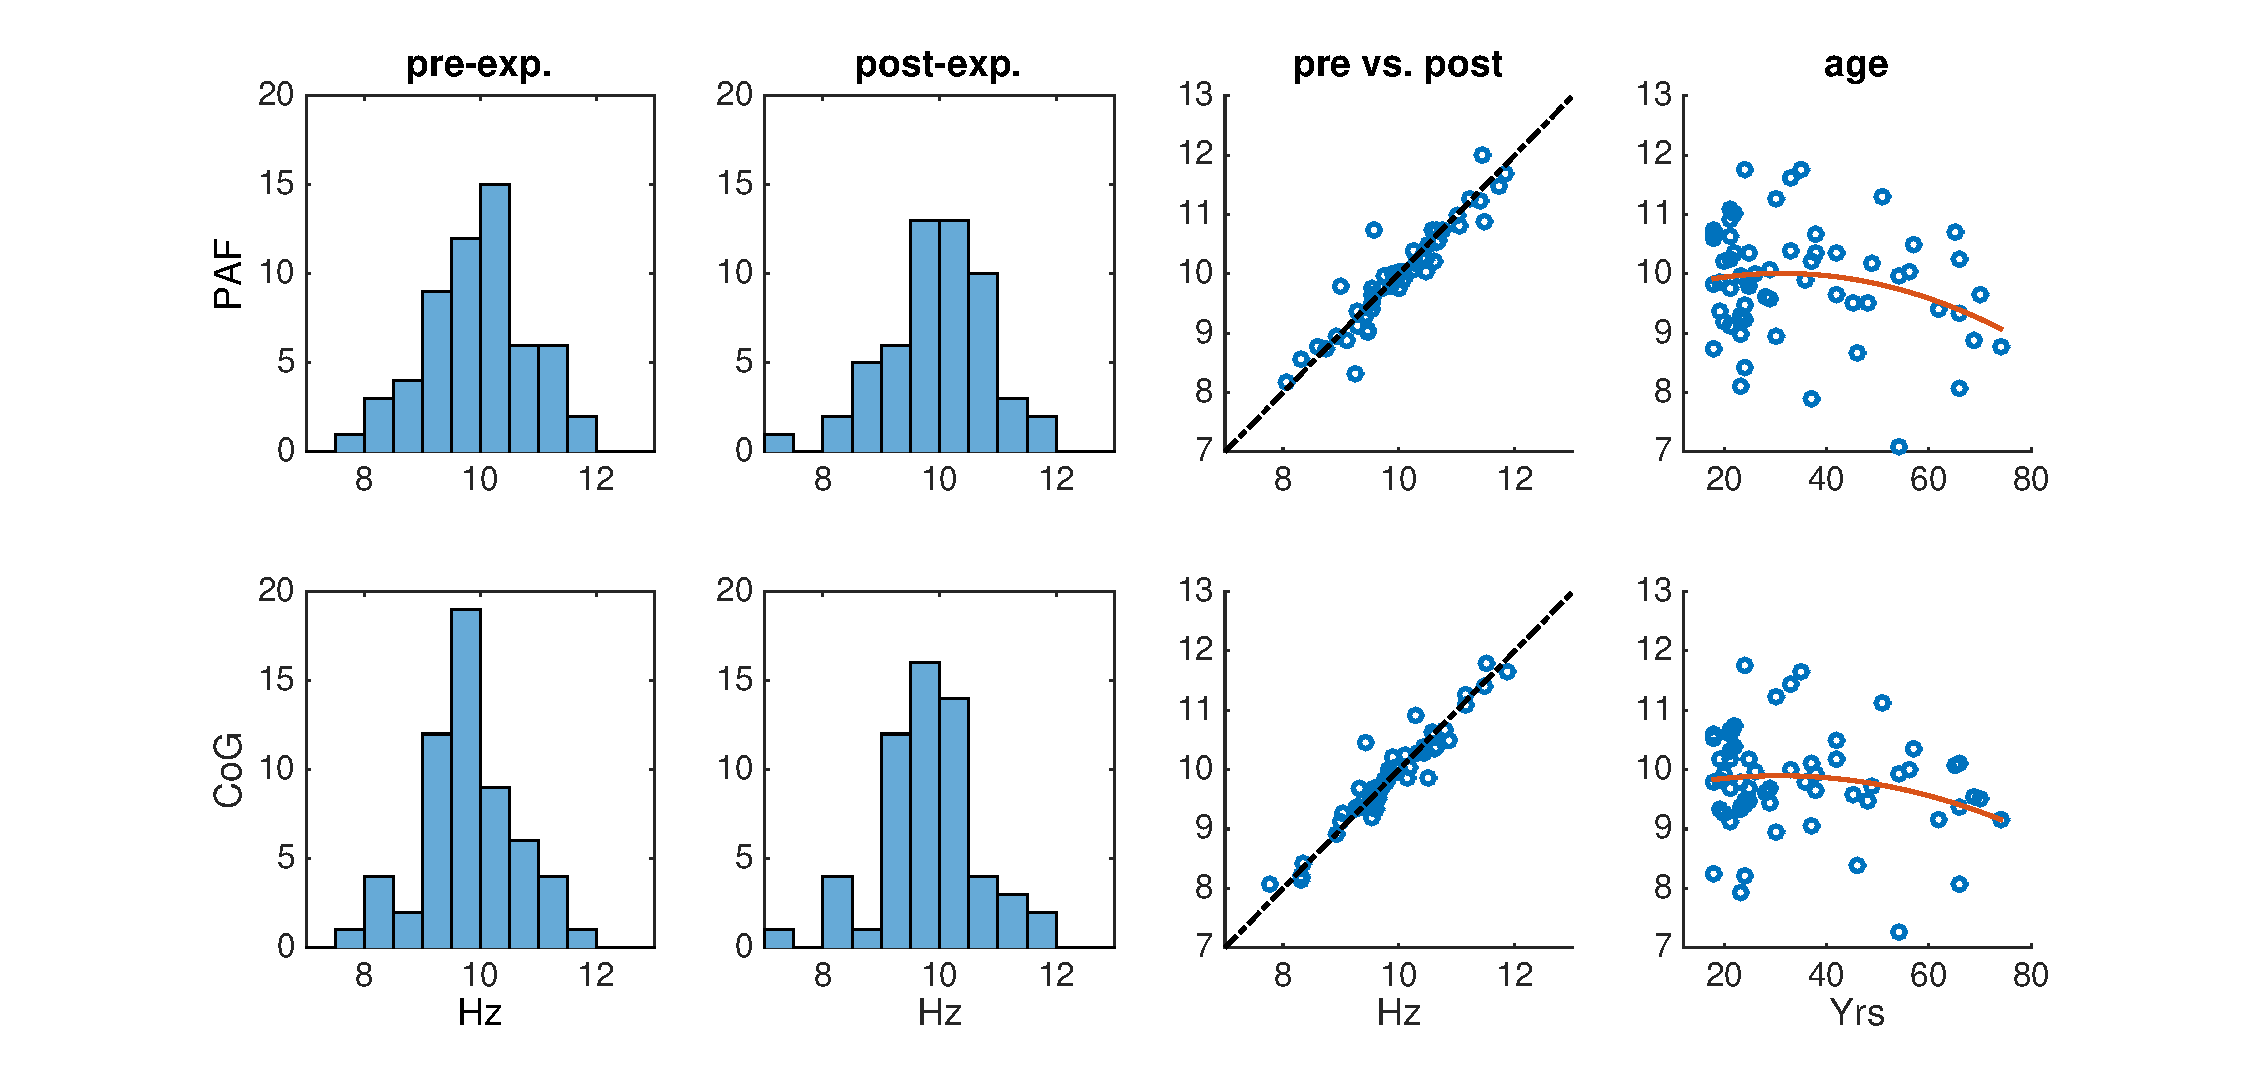
\includegraphics[clip, trim=1cm 0cm 1cm 0cm, width=\textwidth]{empir.eps}
\hrule
\medskip
\includegraphics[clip, trim=1.5cm 0cm 1.5cm 0cm, width=0.5\textwidth]{snr_015.eps}
\includegraphics[clip, trim=1.4cm 0cm 1.4cm 0cm, width=0.5\textwidth]{snr_040.eps}

}

\headerbox{Conclusions}{name=conc,column=2,below=results}{
-- S-G filtering aids accurate, automated extraction of target alpha components.
\\-- Empirical data show similar characteristics to previous large \emph{n} studies.
\\-- \emph{restingIAF} may help improve reliability and rigour of future IAF research.

}

\headerbox{Future Work}{name=affils,column=3,below=results}{
  \begin{todolist}[noitemsep]
  \item \textbf{\textsc{Soon:}}
  \item[--] GitHub release
  \item[--] Assess performance in children
  \item \textbf{\textsc{Later:}}
  \item[--] Develop GUI for EEGLAB
  \item[--] Automate S-G filter settings
  \end{todolist}
}

\headerbox{Affiliations \& References}{name=refs,span=2,column=2,below=conc}{
\smaller[2]{
\textsuperscript{a}Cognition \& Philosophy Laboratory, Monash University.
\textsuperscript{b}Cognitive Neuroscience Laboratory, University of South Australia.
\textsuperscript{c}Max Planck Institute for Psycholinguistics, Nijmegen.}
\textbf{\textsc{Contact}: andrew.corcoran1@monash.edu}

\smaller[2]
[1] Cecere et al. \emph{Curr. Biol.} \textbf{2015}, \emph{25}, 231.
[2] Samaha \& Postle. \emph{Curr. Biol.} \textbf{2015}, \emph{25}, 2985.
[3] Klimesch. \emph{Brain Res. Rev.} \textbf{1999}, \emph{29}, 169.
[4] MacLean et al. \emph{Brain Cogn.} \textbf{2012}, \emph{78},{\vspace{-\baselineskip} 218.
[5] Bornkessel et al. \emph{Exp. Psychol.} \textbf{2004}, \emph{51}, 279.
[6] Grandy et al. \emph{NeuroImage.} \textbf{2013}, \emph{79}, 10.
[7] Klimesch. \emph{TICS.} \textbf{2012}, \emph{16}, 606.
[8] Zeigler. \emph{Appl. Spectrosc.} \textbf{1981}, \emph{35}, 88.}
}

\end{poster}

\end{document}